\documentclass[12pt,a4paper]{article}

\makeatletter
\def\input@path{{/home/maenwe/Master_CSM/modèle_cours_latex}}
\makeatother

\setlength{\spaceskip}{0.3em} %taille inter-mot

\usepackage{prise_de_note}

\geometry{
	margin=1cm,
	top=-.2cm,
	bottom=-.5cm
}

\thispagestyle{empty} 

\newcommand{\Lean}{\textsf{L}\kern-0.1em$\bm{\exists}$\kern-0.1em$\bm\forall$\textsf{N}}
\newcommand{\taille}[3][10pt]{{\fontsize{#2}{#1}\selectfont #3}} % Taille du texte #1 définit l'interligne et par défaut est définie à 10pt
\newcommand{\saut}[1][1cm]{\vspace{#1}} %Saut de ligne

\newcommand{\MasterCSM}[1]{\href{https://formations.univ-rennes.fr/parcours/master-mention-mathematiques-et-applications-parcours-calcul-scientifique-et-modelisation}{#1}}

\begin{document}
	\newlength{\petit}
	\setlength{\petit}{.5cm}
	
	
	%BANDEAU VERTICAL A GAUCHE
	\noindent\fcolorbox{white}{orange!80}{%
		\begin{minipage}[t][0.97\paperheight]{6.1cm}
			$ $
			
			\vspace{6cm}
			
			\begin{center}
				\taille{11pt}{
					\blanc{\textbf{DIPLÔMES/CONCOURS}}}
				\taille{10pt}{
					\blanc{Master, Agrégation}}
				
				\saut
				
				\taille{11pt}{
					\blanc{\textbf{LANGUES}}}\\
				\taille{10pt}{
					\blanc{Anglais (courant)}}
				
				\saut
				
				\taille{11pt}{
					\blanc{\textbf{PASSIONS}}}
				
				\vspace{.4cm}
				
				\hspace{-1.8cm}\begin{minipage}{5.7cm}
					\begin{enumerate}[itemsep=-.5em, align=left]
						\item[{\taille{10pt}{\blanc{Mathématiques :}}}]{\linespread{.7}\selectfont % espace inter-ligne (local)
							$ $\\					
							\blanc{\simplebar{\setlength{\spaceskip}{0.2em} % espace inter-mot
									\taille{9pt}{Étude en temps libre :}\\
									\hspace*{.2cm} \begin{minipage}[t]{15cm}
										\taille{9pt}{Algèbre :} \begin{minipage}[t]{10cm}\taille{9pt}{
												Théorie des représentations\\
												Théorie de homologie\\
												Géométrie algébrique\\
												Géométrie riemannienne}
										\end{minipage}\\\\
										\taille{9pt}{Analyse :} \begin{minipage}[t]{5cm}\taille{9pt}{
												Théorie de Fourier\\
												Analyse fonctionnelle}
										\end{minipage}\\
										\taille{9pt}{\Lean :} \taille{9pt}{\href{https://adam.math.hhu.de/}{\underline{lean4game}}}
									\end{minipage}
						}}}
						
						
						\item[{\taille{10pt}{\blanc{Informatique :}}}]{\linespread{.7}\selectfont % espace interligne (local)
							$ $\\					
							\blanc{\simplebar{\setlength{\spaceskip}{0.2em} % espace inter-mot
									\hspace*{.05cm}\begin{minipage}[t]{5.8cm}
										\taille{9pt}{Création de jeu de plateau basé sur \Lean\\
											Réseaux de neurones}
									\end{minipage}
						}}}
						
						\item[{\taille{10pt}{\blanc{Entomologie}}}]
						
						\item[{\taille{10pt}{\blanc{Astronomie :}}}]{\linespread{.7}\selectfont % espace interligne (local)
							$ $\\					
							\blanc{\simplebar{\setlength{\spaceskip}{0.2em} % espace inter-mot
									\hspace*{.05cm}\begin{minipage}[t]{5.7cm}
										\taille{9pt}{Pratiqué avec un Skywatcher 120/1000}
									\end{minipage}
						}}}
						
						\item[{\taille{10pt}{\blanc{Electronique}}}]
						
						\item[{\taille{10pt}{\blanc{Bricolage}}}]
						
						\item[{\taille{10pt}{\blanc{Lecture}}}]
					\end{enumerate}
				\end{minipage}
				
				\saut[1.3cm]
				
				\taille{11pt}{
					\blanc{\textbf{SPORT \& LOISIR}}}
				
				\vspace{.4cm}
				
				\hspace*{-.7cm}\begin{minipage}{7cm}\begin{spacing}{0.9}
						
						\begin{enumerate}[itemsep=-.5em, align=left]
							\item[{\taille{10pt}{\blanc{Piano :}}}]{\setlength{\spaceskip}{0.2em} % espace inter-mot
								$ $\\
								\blanc{\simplebar{
										\taille{9pt}{Depuis 16 ans, répertoire classique}				
							}}}
							
							\item[{\taille{10pt}{\blanc{Aviron :}}}]{\setlength{\spaceskip}{0.2em} % espace inter-mot
								$ $
								
								\vspace{.1cm}
								
								\blanc{\simplebar{
										\taille{9pt}{5 ans en compétitions et une fois
											en championnat de France}				
							}}}
							
						\end{enumerate}
					\end{spacing}
				\end{minipage}
				
				\saut
				
				\taille{11pt}{
					\blanc{\textbf{VOYAGES}}}\\
				\taille{10pt}{
					\blanc{Angleterre, Irlande, Inde, Italie}}
				
				\saut
				
				\taille{11pt}{
					\blanc{\textbf{PERMIS B}}}
			\end{center}
	\end{minipage}}
	
	\vspace{-28.5cm}
	
	% BANDEAU DU HAUT
	$ $\hspace*{2cm}\begin{minipage}{17cm}
		\begin{tcolorbox}[
			colframe=white,
			colback=orange!40,
			arc=3mm,
			boxrule=.2cm,
			left=6pt,
			right=6pt,
			top=6pt,
			bottom=6pt
			]
			
			\begin{minipage}{6cm}
				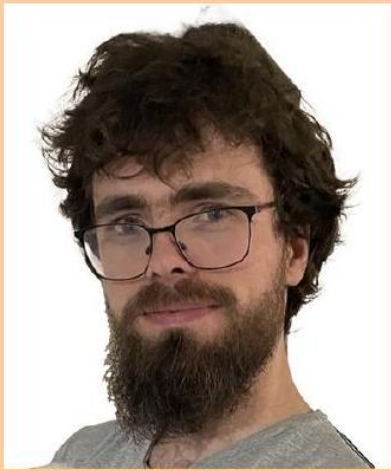
\includegraphics[scale=.25]{photo.png}
			\end{minipage}\begin{minipage}{10cm}
				{\fontsize{26pt}{13pt}\selectfont
					\blanc{\textbf{Nathan HASCOËT}}
				}\\
				{\fontsize{13pt}{13pt}\selectfont
					\blanc{Etudiant en mathématiques appliquées :}
				}\\
				{\fontsize{9pt}{13pt}\selectfont
					\blanc{Parcours}
				}{\fontsize{10.5pt}{13pt}\selectfont \blanc{\underline{\MasterCSM{Calcul Scientifique et Modélisation}}}}
				
				\vspace{.3cm}
				
				\newcommand{\Linkedin}[1]{\href{https://fr.linkedin.com/in/nathan-hascoët-880067264}{#1}}
				\newcommand{\mail}[1]{\href{mailto:nathan-h@laposte.net}{#1}}
				
				\begin{minipage}{1cm}
					
\includegraphics[scale=.07]{linkedin.png}
				\end{minipage}\begin{minipage}{10cm}
					\fontsize{10pt}{13pt}\selectfont
					\blanc{\underline{\Linkedin{Linkedin Nathan Hascoët}}}
				\end{minipage}
				
				\begin{minipage}{1cm}
					
\includegraphics[scale=.3]{phone.png}
				\end{minipage}\begin{minipage}{10cm}
					\fontsize{10pt}{13pt}\selectfont
					\blanc{06 95 87 57 93}
				\end{minipage}
				
				\begin{minipage}{1cm}
					
\includegraphics[scale=.3]{mail.png}
				\end{minipage}\begin{minipage}{10cm}
					\fontsize{10pt}{13pt}\selectfont
					\blanc{\underline{\mail{nathan-h@laposte.net}}}
				\end{minipage}
				
			\end{minipage}
		\end{tcolorbox}
	\end{minipage}
	
	\vspace{-.3cm}
	
	%COMPETENCES
	\hspace{5.8cm}
	\begin{minipage}{13cm}
		\begin{minipage}[t]{7.1cm}
			\begin{tcolorbox}[
				colframe=white,
				colback=orange!80,
				arc=3mm,
				boxrule=2pt,
				left=6pt,
				right=6pt,
				top=2pt,
				bottom=2pt
				]
				\begin{center}
					\blanc{\textbf{\taille{12pt}{COMPETENCES}}}
				\end{center}
			\end{tcolorbox}
		\end{minipage}
		
		%LANGAGE DE PROGRAMMATION
		\hspace*{.1cm}
		\begin{minipage}[t]{6.5cm}
			\begin{tcolorbox}[
				colframe=white,
				colback=orange!40,
				arc=2mm,
				boxrule=2pt,
				left=1pt,
				right=1pt,
				top=1pt,
				bottom=1pt
				]
				\blanc{\textbf{\taille{12pt}{Langages de programmation}}}
			\end{tcolorbox}
		\end{minipage}
		
		\vspace{-.5cm}
		
		\hspace*{-.4cm}
		\begin{minipage}[t]{14.5cm}
			\begin{spacing}{.2}	
				\setlength{\spaceskip}{0.2em}		
				\begin{enumerate}[label=$\star$\hspace{-.1cm}]
					\item \taille{10pt}{\underline{C :}} \begin{minipage}[t]{10cm}\taille{9pt}{
							réalisation d’un programme « éléments finis ».\\
							BLAS et LAPACK.}
					\end{minipage}
					
					\item \taille{10pt}{\underline{Python :}} \begin{minipage}[t]{12cm}\taille{9pt}{
							machine learning (algorithme de Kohonen) appliqué à la compression
							
							méthodes statistiques (voir ci-dessous).}
					\end{minipage}
					
					\item \taille{10pt}{\underline{Matlab :}} \begin{minipage}[t]{10cm}\taille{9pt}{
							manipulation de méthodes numériques (voir ci-dessous).\\  
							simulation de la dynamique d’une corde dans le cadre d’un projet.}
					\end{minipage}
					
					\item \taille{10pt}{\underline{Git/github :}} \begin{minipage}[t]{10.5cm}\taille{9pt}{
							projet collaboratif : simulation numérique d’une corde d’après ses caractéristiques physiques.}
					\end{minipage}
					
					\item \taille{10pt}{\underline{\LaTeX :}} \begin{minipage}[t]{10cm}\taille{9pt}{
							prises de notes des cours, rapports.}
					\end{minipage}
					
					
					\item \taille{10pt}{\underline{\href{https://lean-lang.org/}{\Lean}} :}
					\begin{minipage}[t]{10cm}
						\taille{9pt}{\href{https://lean-lang.org/}{assistant de preuves mathématiques (pratique sur mon temps libre).}}
					\end{minipage}
					
					\item \taille{10pt}{\href{https://www.sagemath.org/index.html}{\underline{SageMath :}}} \begin{minipage}[t]{11cm}\taille{9pt}{
							\href{https://www.sagemath.org/index.html}{calcul formel, utilisé pour l’Agrégation de mathématiques.}}
					\end{minipage}
					
					\item \taille{10pt}{\underline{Shell :}} \taille{9pt}{linux, scripting, automatisation}
				\end{enumerate}
			\end{spacing}
		\end{minipage}
		
		%COMPETENCE SCIENTIFIQUE
		\hspace*{.1cm}
		\begin{minipage}[t]{5.8cm}
			\begin{tcolorbox}[
				colframe=white,
				colback=orange!40,
				arc=2mm,
				boxrule=2pt,
				left=1pt,
				right=1pt,
				top=1pt,
				bottom=1pt
				]
				\blanc{\textbf{\taille{12pt}{Compétences scientifiques}}}
			\end{tcolorbox}
		\end{minipage}
		
		\vspace{-.5cm}
		
		\hspace*{-.55cm}
		\begin{minipage}[t]{12.8cm}
			\begin{spacing}{.5}	\setlength{\spaceskip}{0.2em}		
				\begin{enumerate}[label=$\star$\hspace{-.1cm}]
					\item \taille{10pt}{\underline{Statistique :}} 			\begin{minipage}[t]{10cm}\taille{9pt}{
							ACP, clustering, analyse discriminante, régression (linéaire, Ridge, Lasso), approche non paramétrique, agrégation de modèles, deep learning.}
					\end{minipage}	
					
					\item \taille{10pt}{\underline{Méthode numérique :}} 			\begin{minipage}[t]{8.8cm}\taille{9pt}{
							résolution d’EDO, intégration, système linéaire, coup de calcul et estimation d’erreurs.}
					\end{minipage}	
					
					\item \taille{10pt}{\underline{Optimisation :}} 			\begin{minipage}[t]{11cm}\taille{9pt}{
							méthode du gradient, d’Uzawa, du simplexe, problème de transport.}
					\end{minipage}	
					
					\item \taille{10pt}{\setlength{\spaceskip}{0.2em}\underline{Équations aux dérivées partielles :}} \begin{minipage}[t]{8.4cm}
						\taille{9pt}{
							formulations variationnelles, décompositions modales, différences finies, éléments finis.}
					\end{minipage}			
				\end{enumerate}
			\end{spacing}
		\end{minipage}
		
		\saut[.5cm]
		
		
		%FORMATIONS
		\begin{minipage}[t]{7.1cm}
			\begin{tcolorbox}[
				colframe=white,
				colback=orange!80,
				arc=3mm,
				boxrule=2pt,
				left=6pt,
				right=6pt,
				top=2pt,
				bottom=2pt
				]
				\begin{center}
					\blanc{\textbf{\taille{12pt}{FORMATIONS}}}
				\end{center}
			\end{tcolorbox}
			
			\saut[-.4cm]
			
			\hspace{1cm}
			\begin{minipage}[t]{12.5cm}
				\begin{enumerate}[itemsep=-.5em]\setlength{\spaceskip}{0.2em}
					\item[\taille{10pt}{2027 - 2030 :}\hspace{-.1cm}] \taille{10pt}{Doctorat en mathématiques appliqué (Univ. Rennes)}
					
					\item[\taille{10pt}{2025 - 2027 :}\hspace{-.1cm}] \taille{10pt}{\MasterCSM{Master Calcul Scientifique et Modélisation (Univ. Rennes)}}
					
					\item[\taille{10pt}{2023 :}\hspace{-.1cm}] \taille{10pt}{Agrégation externe de mathématiques}
					
					\item[\taille{10pt}{2020 - 2022 :}\hspace{-.1cm}] \taille{10pt}{Master préparation à l’agrégation (Univ. Rennes)}
					
					\item[\taille{10pt}{2019 - 2020 :}\hspace{-.1cm}] \taille{10pt}{Licence de mathématiques pour la recherche (Univ. Rennes)}
					
					\item[\taille{10pt}{2017 - 2019 :}\hspace{-.1cm}]
					\taille{10pt}{Classe préparatoire aux grandes écoles - MPSI (Dupuy de Lôme à Lorient)}
					
					
				\end{enumerate}
			\end{minipage}
		\end{minipage}
		
		\saut[\petit]
		
		%Expérience Pro
		\begin{minipage}[t]{11cm}
			\begin{tcolorbox}[
				colframe=white,
				colback=orange!80,
				arc=3mm,
				boxrule=2pt,
				left=6pt,
				right=6pt,
				top=2pt,
				bottom=2pt
				]
				\begin{center}
					\blanc{\textbf{\taille{12pt}{EXPERIENCES PROFESSIONNELLES}}}
				\end{center}
			\end{tcolorbox}
			
			
			\vspace{-.2cm}
			
			%UNIVERSITE
			\hspace*{.1cm}
			\begin{minipage}[t]{5.8cm}
				\begin{tcolorbox}[
					colframe=white,
					colback=orange!40,
					arc=2mm,
					boxrule=2pt,
					left=1pt,
					right=1pt,
					top=1pt,
					bottom=1pt
					]
					\blanc{\textbf{\taille{12pt}{Université}}}
				\end{tcolorbox}
			\end{minipage}
			
			\vspace{-.2cm}
			
			\hspace{.5cm}\setlength{\spaceskip}{0.2em}\taille{10pt}{Printemps-été 2021 :} \begin{minipage}[t]{10cm}
				\begin{spacing}{.8}
					\taille{10pt}{Stage en géométrie algébrique sous la tutelle de\\
						M. Bernard Le Stum}
				\end{spacing}
			\end{minipage}
			
			\vspace{-.2cm}
			
			%Professeur de mathématiques
			\hspace*{.1cm}
			\begin{minipage}[t]{7cm}
				\begin{tcolorbox}[
					colframe=white,
					colback=orange!40,
					arc=2mm,
					boxrule=2pt,
					left=1pt,
					right=1pt,
					top=1pt,
					bottom=1pt
					]
					\blanc{\textbf{\taille{12pt}{Professeur de mathématiques}}}
				\end{tcolorbox}
			\end{minipage}
			
			\vspace{-.2cm}
			
			\hspace{.5cm}\setlength{\spaceskip}{0.2em}\taille{10pt}{2020 - ... :} \begin{minipage}[t]{10cm}
				\begin{spacing}{.8}
					\taille{10pt}{Professeur particulier de mathématiques}
				\end{spacing}
			\end{minipage}
			
			\vspace{-.2cm}
			
			\hspace{.5cm}\setlength{\spaceskip}{0.2em}\taille{10pt}{2022 - 2025 :} \begin{minipage}[t]{10cm}
				\begin{spacing}{.8}
					\taille{10pt}{Professeur de mathématiques au collège et au lycée}
				\end{spacing}
			\end{minipage}
			
			\vspace{-.2cm}
			
			
			%AUTRE
			\hspace*{.1cm}
			\begin{minipage}[t]{7cm}
				\begin{tcolorbox}[
					colframe=white,
					colback=orange!40,
					arc=2mm,
					boxrule=2pt,
					left=1pt,
					right=1pt,
					top=1pt,
					bottom=1pt
					]
					\blanc{\textbf{\taille{12pt}{Autre}}}
				\end{tcolorbox}
			\end{minipage}
			
			\vspace{-.2cm}
			
			\hspace{.5cm}\setlength{\spaceskip}{0.2em}\taille{10pt}{2022 - 2023 :} \begin{minipage}[t]{10cm}
				\begin{spacing}{.8}
					\taille{10pt}{Technicien de surface}
				\end{spacing}
			\end{minipage}
			
			\vspace{-.2cm}
			
			\hspace{.5cm}\setlength{\spaceskip}{0.2em}\taille{10pt}{Eté 2021 :} \begin{minipage}[t]{10cm}
				\begin{spacing}{.8}
					\taille{10pt}{Déménageur à JSB déménagements à Vern-sur-Seiche}
				\end{spacing}
			\end{minipage}
		\end{minipage}
	\end{minipage}
\end{document}